% -*- mode: latex; mode: flyspell -*-

%%% Local Variables:
%%% TeX-master: "mu2e-36575"
%%% End:

%%%%%%%%%%%%%%%%%%%%%%%%%%%%%%%%%%%%%%%%%%%%%%%%%%%%%%%%%%%%%%%%%%%%%%%%%%%%%%
\section{Particle Identification}

Datasets used for MVA training : {\bf ele00s61b0} and {\bf mumi0s61b0}


\subsection {Event selection}

After the reconstructed calorimeter cluster is included into the track fit, it biases the fit results.

Something ( a bug?) in the track fit pulls the track timing to the cluster and biases
the reconstructed track timing.

There  is a correlation between the cluster timing residual and the reconstructed Z-coordinate of the
``calorimeter cluster hit'', which the fitter varies in order to minimize the timing residual.

As inclusion of the cluster into the track fit stabilizes the fit and improves its efficiency,
we use track fits with the calorimeter cluster included.

\subsection {Training}

MVA classifiers were trained only for DAR resolver, however based on the nature of 
the variables used, we expect the trained MVA to perform equally well for PAR tracks.

Although both electron and muon reconstruction were ran on the same event, the MVA training used inputs 
only fotm electron reconstruction. Adding requirement for a track to be reconstructed under muon hypothesis 
complicates logic, reduces overall efficiency without providing a visible improvement.

For training: events which have a track reconstructed under DEM\_DAR hypothesis and passing the track 
selection cuts described in 

Variables and their ranking:

\begin{itemize}
\item 
  E(cluster)/P(track) : to reduce explicit dependence on the track momentum 
\item 
  number of crystals in the calorimeter cluster
\item 
  eSeedfr: fraction of energy in the seed crystal
\item 
  $\Delta T$ : time residual of the calorimeter cluster as determined by the kalman fit
\item 
  $Cluster Z$ : cluster Z-coordinate (within the corresponding calorimeter disk) as determined by the kalman fit
\item 
  $\Delta R$ : radial residual of the calorimeter cluster as determined by the kalman fit
\item 
  {\bf path} : overall length of the trajectory within the calorimeter disk, defines edges
\end{itemize}

We didn't consider pathological cases with muons passing electron reconstruction, but failing
the muon one, and assume the probability of that to be negligibly small.

\begin{figure}
\hspace{-1.4in}
\begin{tikzpicture}
  \node[anchor=south west,inner sep=0] at (-1,0.) {
    % \node[shift={(0 cm,0.cm)},inner sep=0,rotate={90}] at (0,0) {}
    % \makebox[\textwidth][c] {
    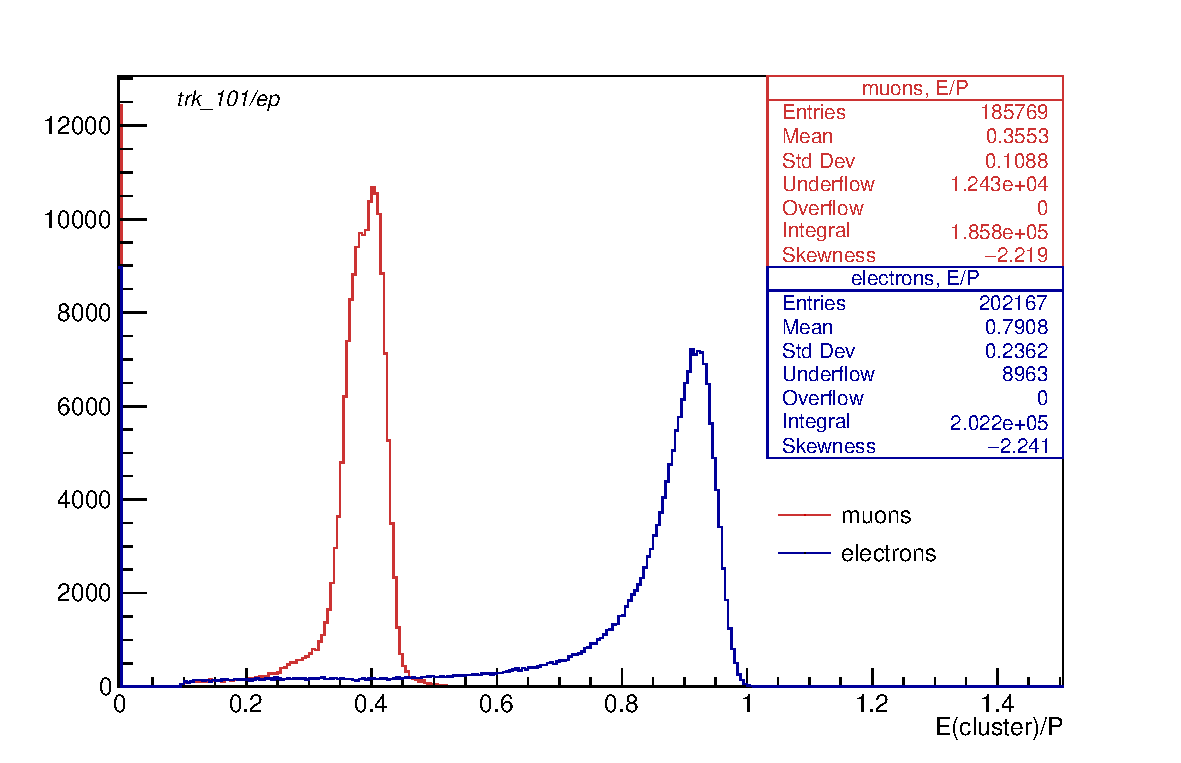
\includegraphics[width=0.80\textwidth]{figures/pdf/figure_00300_pid_emuana_1070_trk_101_ep}
    % }
  };
  \node[anchor=south west,inner sep=0] at (9.5,0.) {
    % \node[shift={(0 cm,0.cm)},inner sep=0,rotate={90}] at (0,0) {}
    % \makebox[\textwidth][c] {
    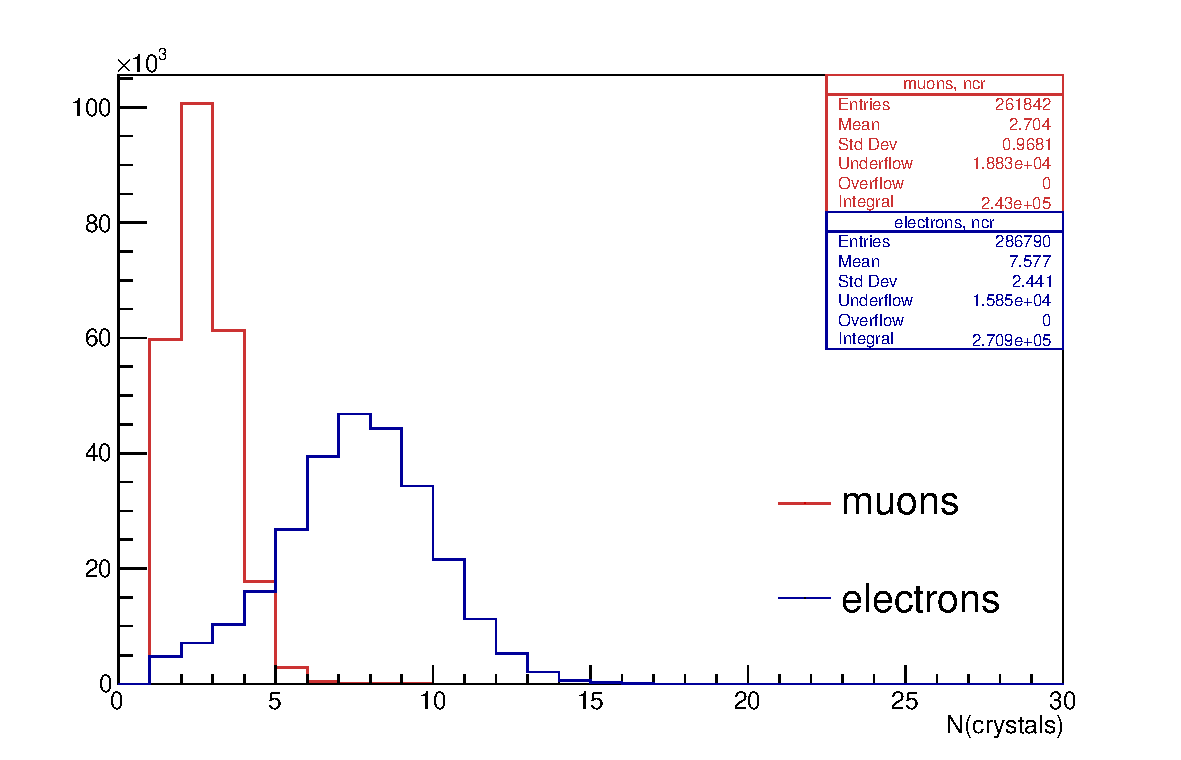
\includegraphics[width=0.80\textwidth]{figures/pdf/figure_00301_pid_emuana_1070_trk_101_ncr}
    % }
  };
  \node[anchor=south west,inner sep=0] at (-1,-6.5) {
    % \node[shift={(0 cm,0.cm)},inner sep=0,rotate={90}] at (0,0) {}
    % \makebox[\textwidth][c] {
    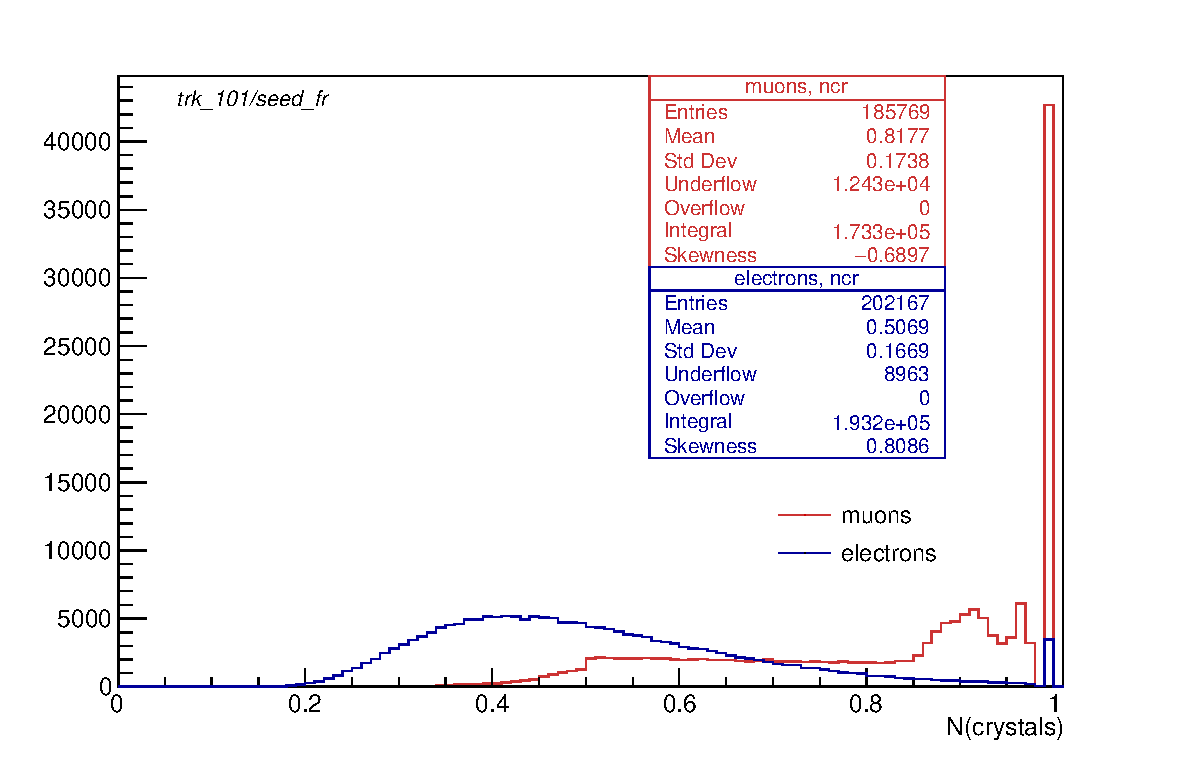
\includegraphics[width=0.80\textwidth]{figures/pdf/figure_00302_pid_emuana_1070_trk_101_seed_fr}
    % }
  };
  \node[anchor=south west,inner sep=0] at (9.5,-6.5) {
    % \node[shift={(0 cm,0.cm)},inner sep=0,rotate={90}] at (0,0) {}
    % \makebox[\textwidth][c] {
    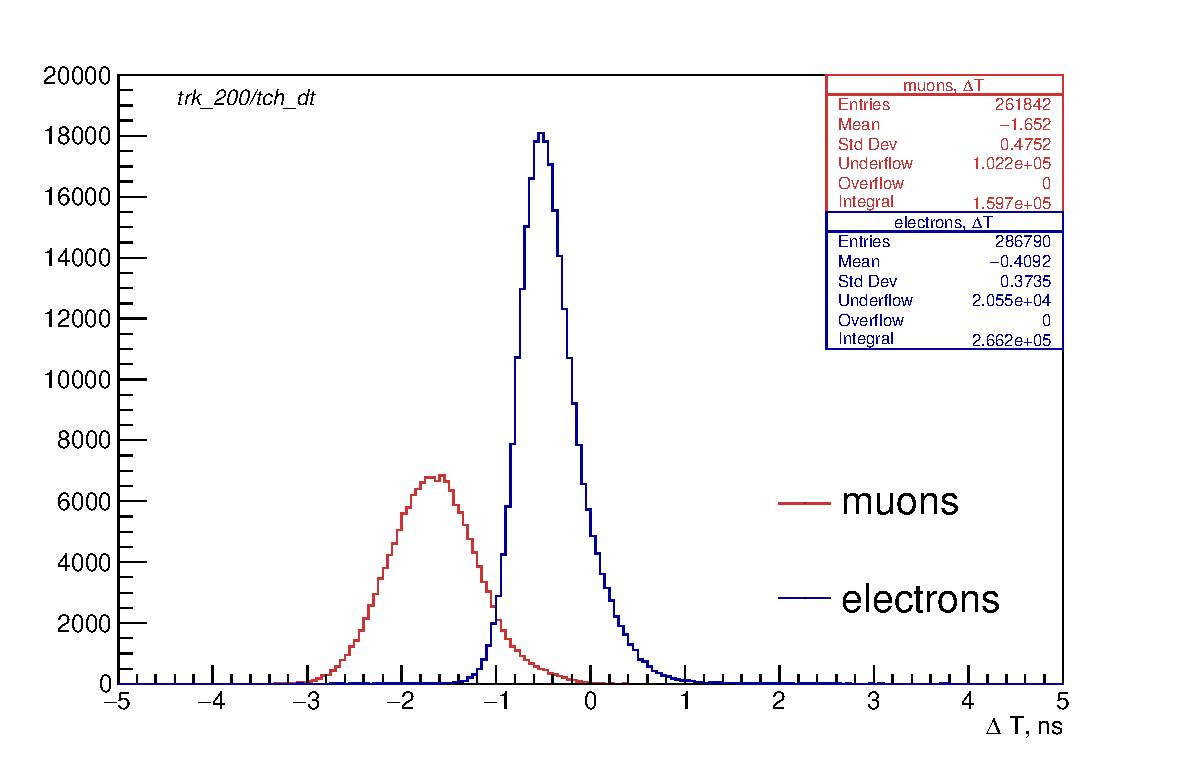
\includegraphics[width=0.80\textwidth]{figures/pdf/figure_00303_pid_emuana_1070_trk_101_tch_dt}
    % }
  };
  \node[anchor=south west,inner sep=0] at (-1,-13.) {
    % \node[shift={(0 cm,0.cm)},inner sep=0,rotate={90}] at (0,0) {}
    % \makebox[\textwidth][c] {
    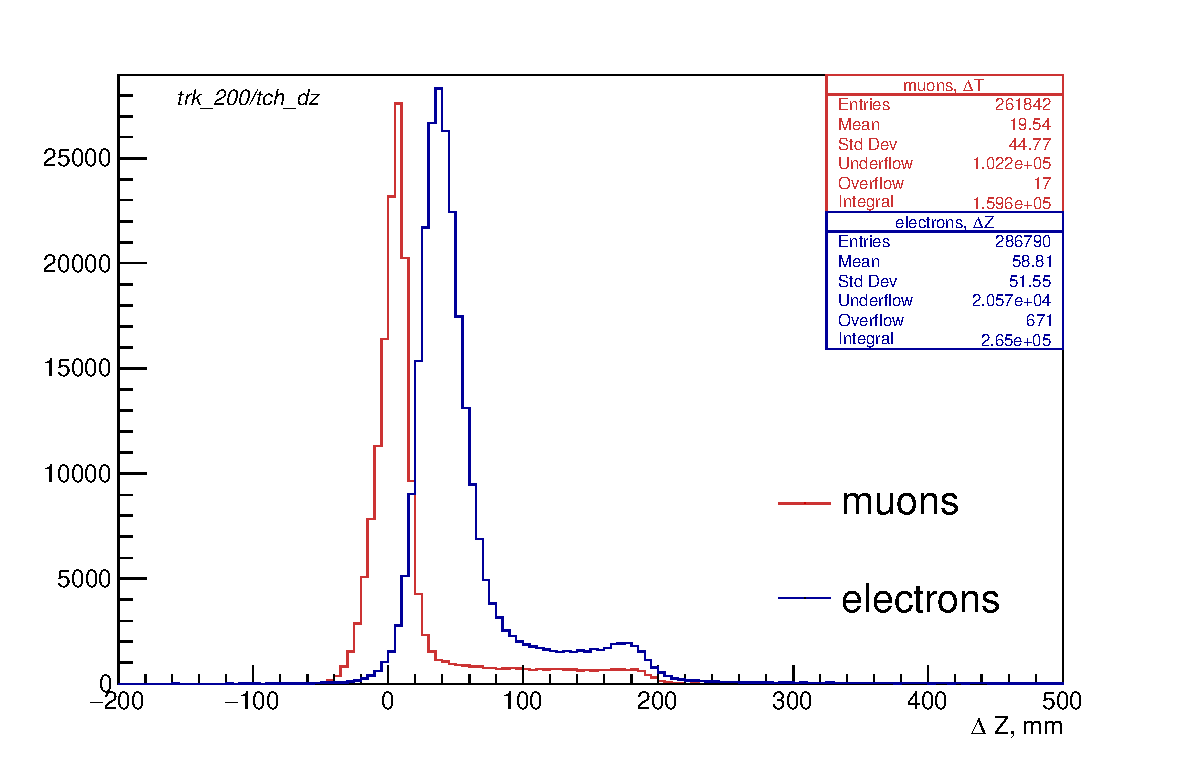
\includegraphics[width=0.80\textwidth]{figures/pdf/figure_00304_pid_emuana_1070_trk_101_tch_dz}
    % }
  };
  \node[anchor=south west,inner sep=0] at (9.5,-13.) {
    % \node[shift={(0 cm,0.cm)},inner sep=0,rotate={90}] at (0,0) {}
    % \makebox[\textwidth][c] {
    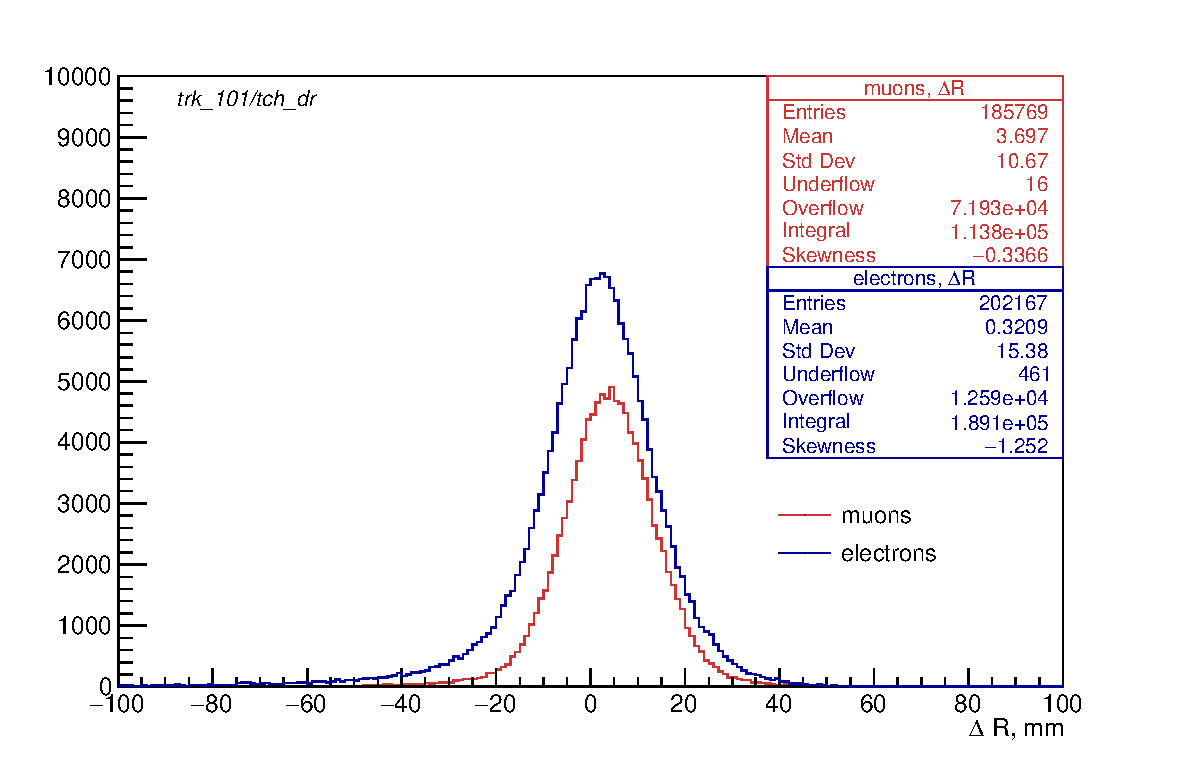
\includegraphics[width=0.80\textwidth]{figures/pdf/figure_00305_pid_emuana_1070_trk_101_tch_dr}
    % }
  };
  % \node [text width=6cm, scale=0.8] at (4.5,6.4) {mu2e-18894 by Kevin Lynch and Jim Popp};
\end{tikzpicture}
% \captionof{figure} {
\caption{
  \label{fig:pid_training_1}
  variables used in PID MVA training
}
\end{figure}

5000 electron and 5000 muon tracks have been used for trainign

Training preselection cuts:

\begin{itemize}
\item 
  reject muon decays in flight: require muon Zmax > 10000,
\item 
  reconstructed track passed electron track selection
\item 
  an event has a reconstructed cluster 
\item 
  $\Delta T > -100$ : some events with reconstructed tracks and clusters had $\Delta T$ undefined
\end{itemize}

\begin{figure}
  \label{fig:pid_training_2}
  \begin{tikzpicture}
    \node[anchor=south west,inner sep=0] at (0,0.) {
      % \node[shift={(0 cm,0.cm)},inner sep=0,rotate={90}] at (0,0) {}
      % \makebox[\textwidth][c] {
      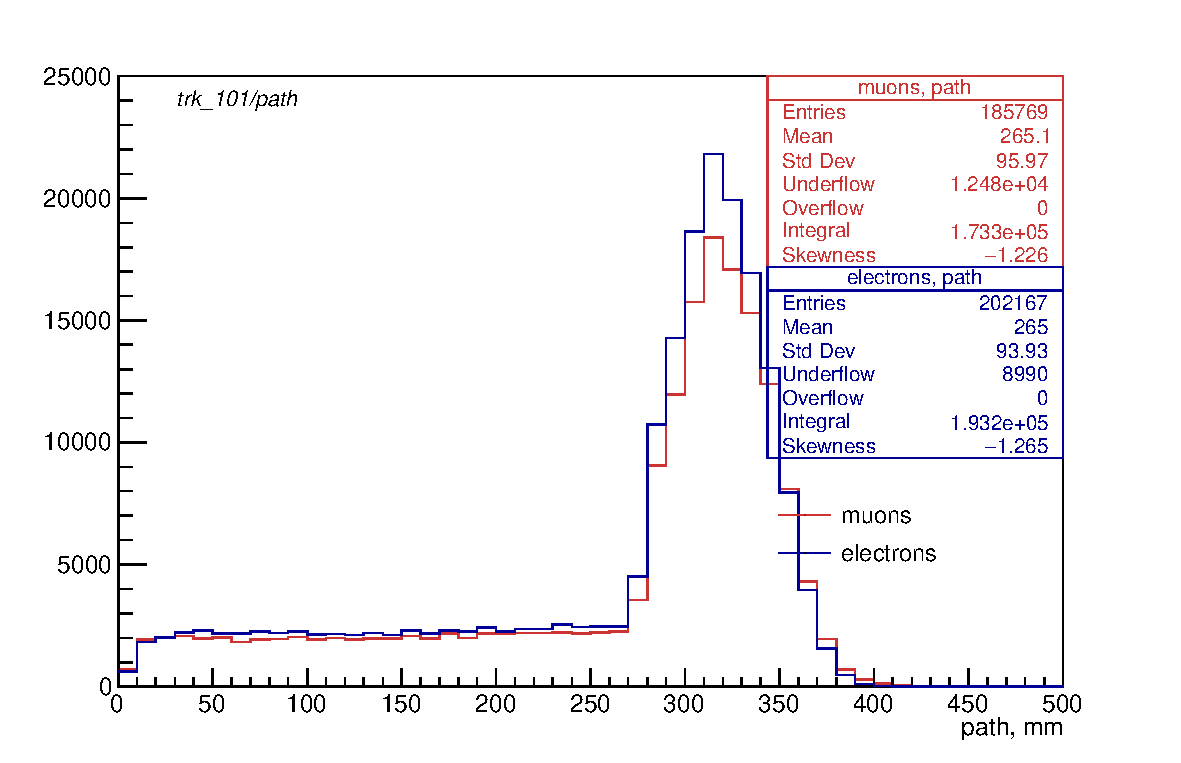
\includegraphics[width=0.8\textwidth]{figures/pdf/figure_00306_pid_emuana_1070_trk_101_path}
      % }
    };
    % \node [text width=6cm, scale=0.8] at (4.5,6.4) {mu2e-18894 by Kevin Lynch and Jim Popp};
  \end{tikzpicture}
  % \captionof{figure} {
  \caption{
    variables used in PID MVA training: particle path in the disk
  }
\end{figure}


training plots :

\begin{figure}
  \label{fig:pid_training_2}
\hspace{-1.4in}
  \begin{tikzpicture}
    \node[anchor=south west,inner sep=0] at (0,0.) {
      % \node[shift={(0 cm,0.cm)},inner sep=0,rotate={90}] at (0,0) {}
      % \makebox[\textwidth][c] {
      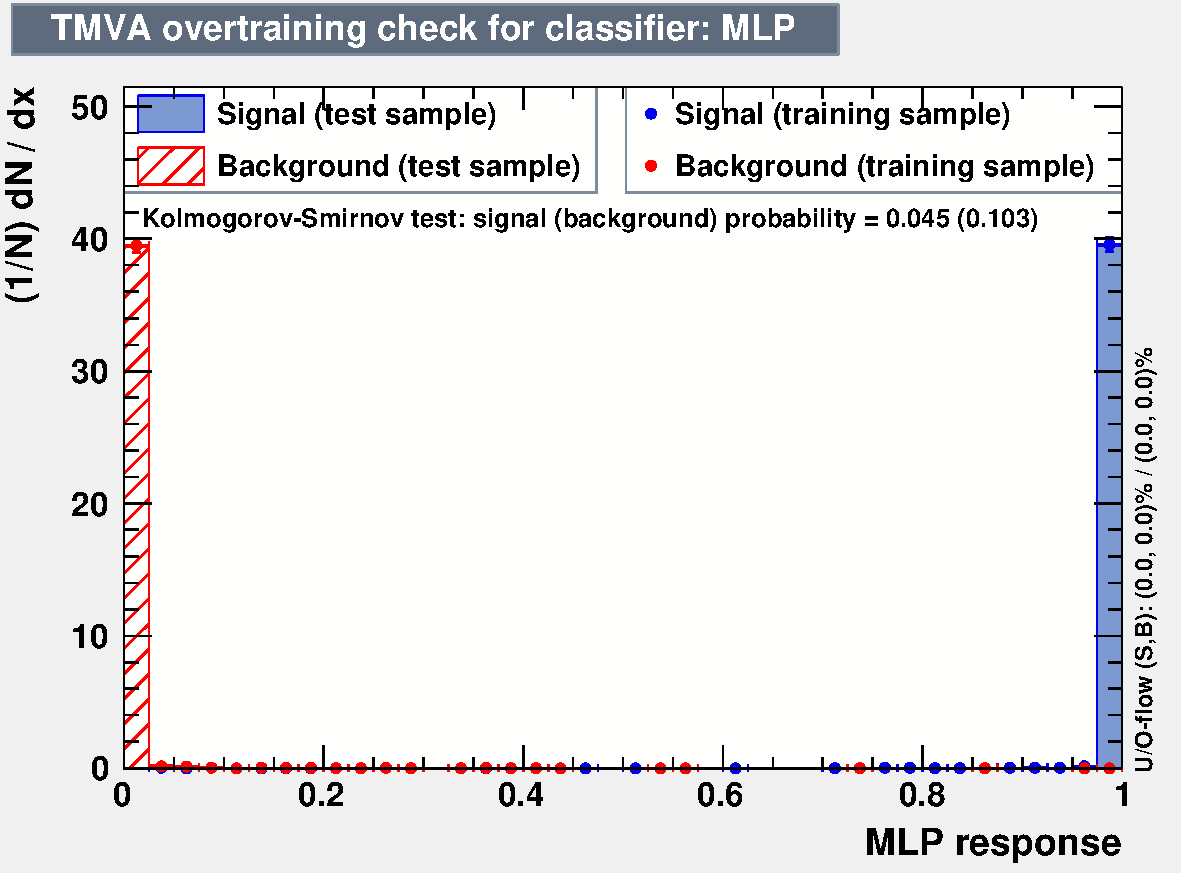
\includegraphics[width=0.70\textwidth]{figures/pdf/pid_mva_overtrain_mlp}
      % }
    };
    \node[anchor=south west,inner sep=0] at (10,0.5) {
      % \node[shift={(0 cm,0.cm)},inner sep=0,rotate={90}] at (0,0) {}
      % \makebox[\textwidth][c] {
      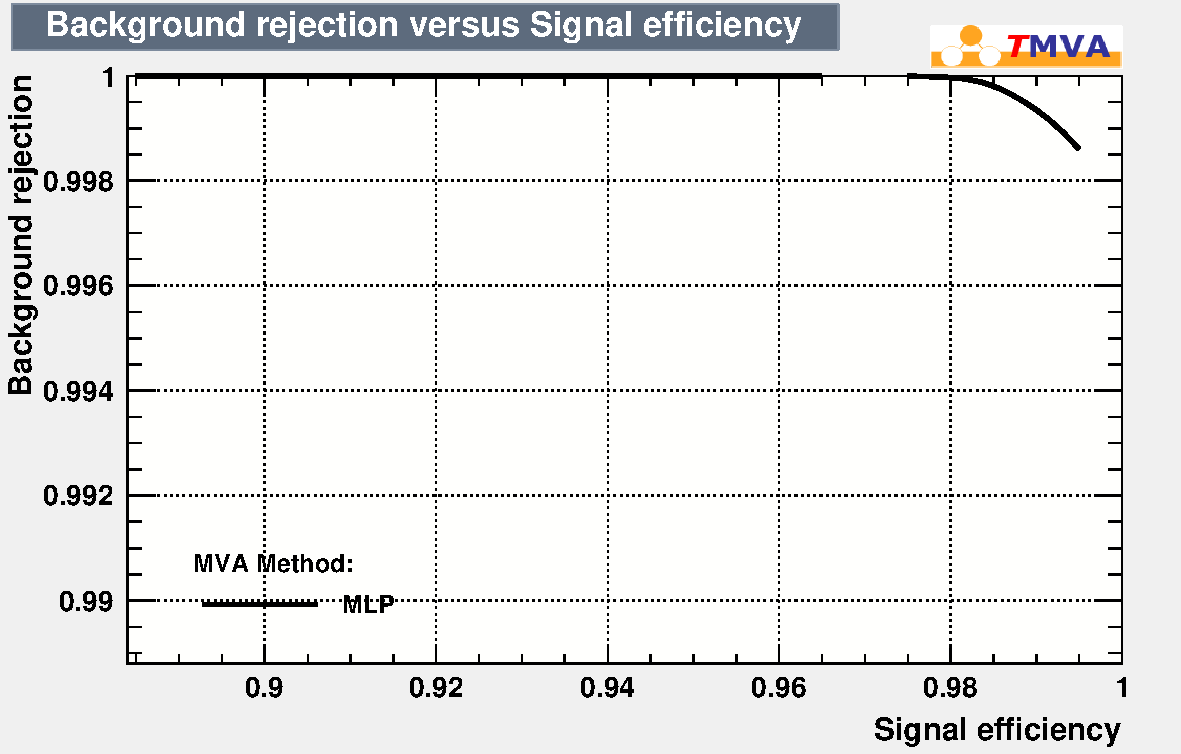
\includegraphics[width=0.70\textwidth]{figures/pdf/pid_mva_rejection_mlp}
      % }
    };
    % \node [text width=6cm, scale=0.8] at (4.5,6.4) {mu2e-18894 by Kevin Lynch and Jim Popp};
  \end{tikzpicture}
  % \captionof{figure} {
  \caption{
    output of the PID ANN training: overtraining check on the left and efficiency vs rejection 
    on the right
  }
\end{figure}



\begin{figure}
  \label{fig:pid_training_2}
  \begin{tikzpicture}
    \node[anchor=south west,inner sep=0] at (0,0.) {
      % \node[shift={(0 cm,0.cm)},inner sep=0,rotate={90}] at (0,0) {}
      \makebox[\textwidth][c] {
        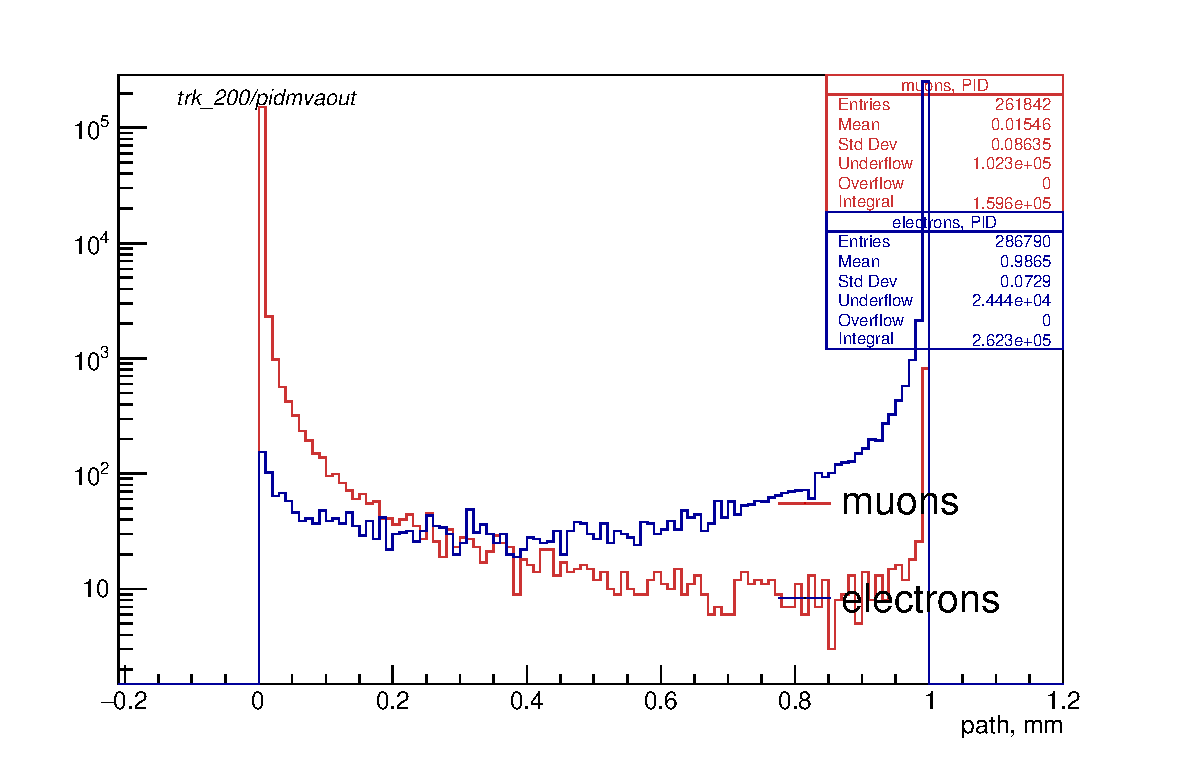
\includegraphics[width=1.0\textwidth]{figures/pdf/figure_00307_pid_emuana_1070_trk_101_pidmvaout}
      }
    };
    % \node [text width=6cm, scale=0.8] at (4.5,6.4) {mu2e-18894 by Kevin Lynch and Jim Popp};
  \end{tikzpicture}
  % \captionof{figure} {
  \caption{
    Distribution in the PID ANN score for electron and muon samples, samples include events used for training,
    5000 events each. A spike in muon PID at 1  - muon decays in flight. \\ 
    {\color{red} \bf Origin of the plotted underflow bin to be investigated}
  }
\end{figure}

PID preselection cuts (ele00s61b0), for reference:

\begin{table}[h!]
  \begin{center}
    \caption{Final Track quality selection}
    \label{tab:table1}
    \begin{tabular}{l|c|c} % <-- Changed to S here.
      \textbf{Cut}                    & \textbf{N events after } & \textbf{Efficiency }\\
      \hline
      Number generated events         & 1000000          &            \\
      total number of tracks          &  329715          &   0.330    \\
      \hline
      track passes TID cuts           &  193252          &   0.586    \\
      $P > 100$                       &  178078          &   0.921    \\
      $|DR| < 100$ mm                 &  167028          &   0.938    \\
      $|DT| < 10$ ns                  &  167028          &   1.0      \\
      $-50 < dz < 250$                &  164951          &   0.988    \\
      $ E/P < 1.2$                    &  164884          &   1.000    \\
      \hline
      $PID >0.5$                      &  163543          &   0.992    \\
   \end{tabular}
  \end{center}
  \caption{
    PID preselection cuts (ele00s61b0) and efficiency for {\bf cele0s51b1} electrons 
  }
\end{table}

Total efficiency of the PID preselection cuts - 0.926. 

Out of that, approximately, 0.958 comes from the requirement of a calorimeter cluster E > 10 MeV to be reconstructed.

Thus, for events with P>100 and a reconstructed cluster, efficiency of the PID preselection - 0.967.

for electron events with the reconstructed track momentum $P > 100$ MeV/c, passing the preselections, 
the PID efficiency is 0.993


Efficiency for muon events passing the same preselections: 

\begin{itemize}
\item
  $P > 100$                       : 109004
\item 
  $PID >0.5$                      :    799
\end{itemize}

which is about 0.8\%.

Contributing to muon mis-identification are decays of stopped muons with in the calorimeter, 
early part of the decay timing exponential, in which the electron energy is counted as the part 
of the cluster energy. 



%%%%%%%%%%%%%%%%%%%%%%%%%%%%%%%%%%%%%%%%%%%%%%%%%%%%%%%%%%%%%%%%%%%%%%%%%%%%%%
\subsection { Electrons, failing the PID selection} 

Figure \ref{fig:electrons_failing_pid} compares distributions in some ID variables for electrons 
passing and failing the PID cuts.

Although only 0.8\% Of events are in question, understanding of the ANN failures could help finding 
reconstruction problems.

Of special interest seems to be the spike in the distribution in R(max)

\begin{figure}
\hspace{-1.4in}
  \begin{tikzpicture}
    \node[anchor=south west,inner sep=0] at (0,0.) {
      % \node[shift={(0 cm,0.cm)},inner sep=0,rotate={90}] at (0,0) {}
      % \makebox[\textwidth][c] {
      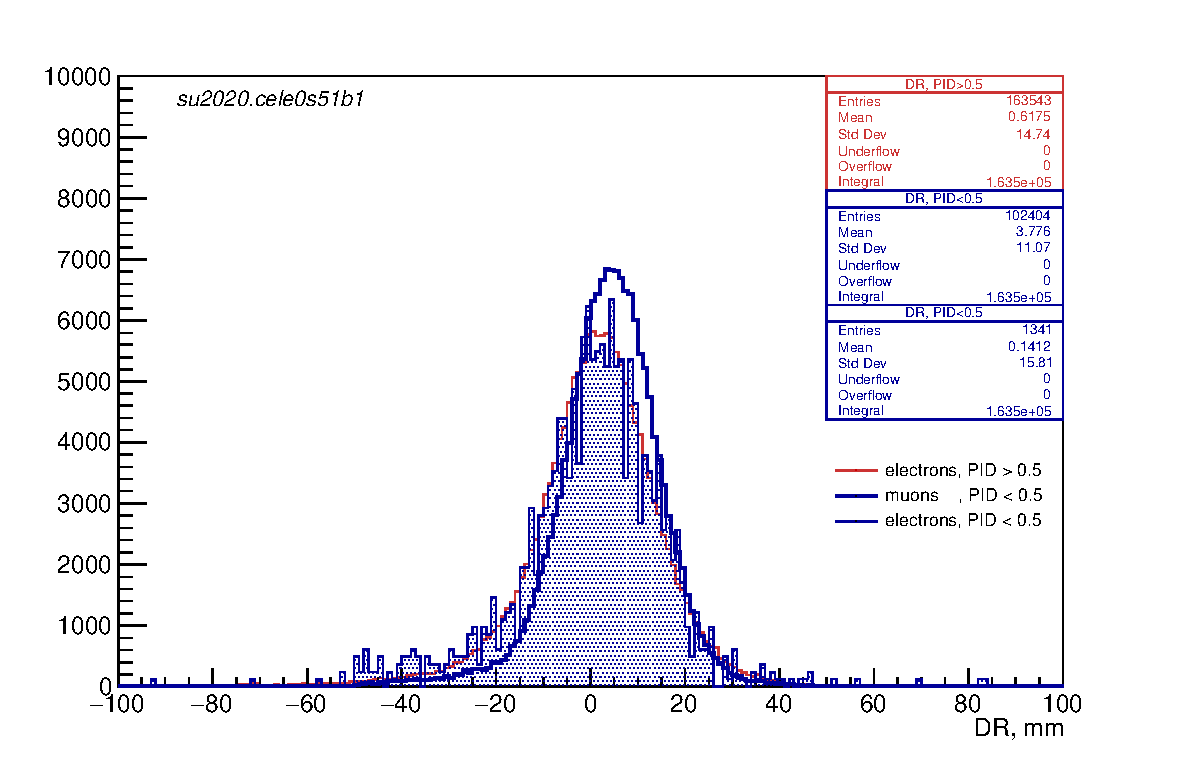
\includegraphics[width=0.80\textwidth]{figures/pdf/figure_00310_pid_emuana_trk_110_vs_111_tch_dr}
      % }
    };
    \node[anchor=south west,inner sep=0] at (10.3,0.) {
      % \node[shift={(0 cm,0.cm)},inner sep=0,rotate={90}] at (0,0) {}
      % \makebox[\textwidth][c] {
      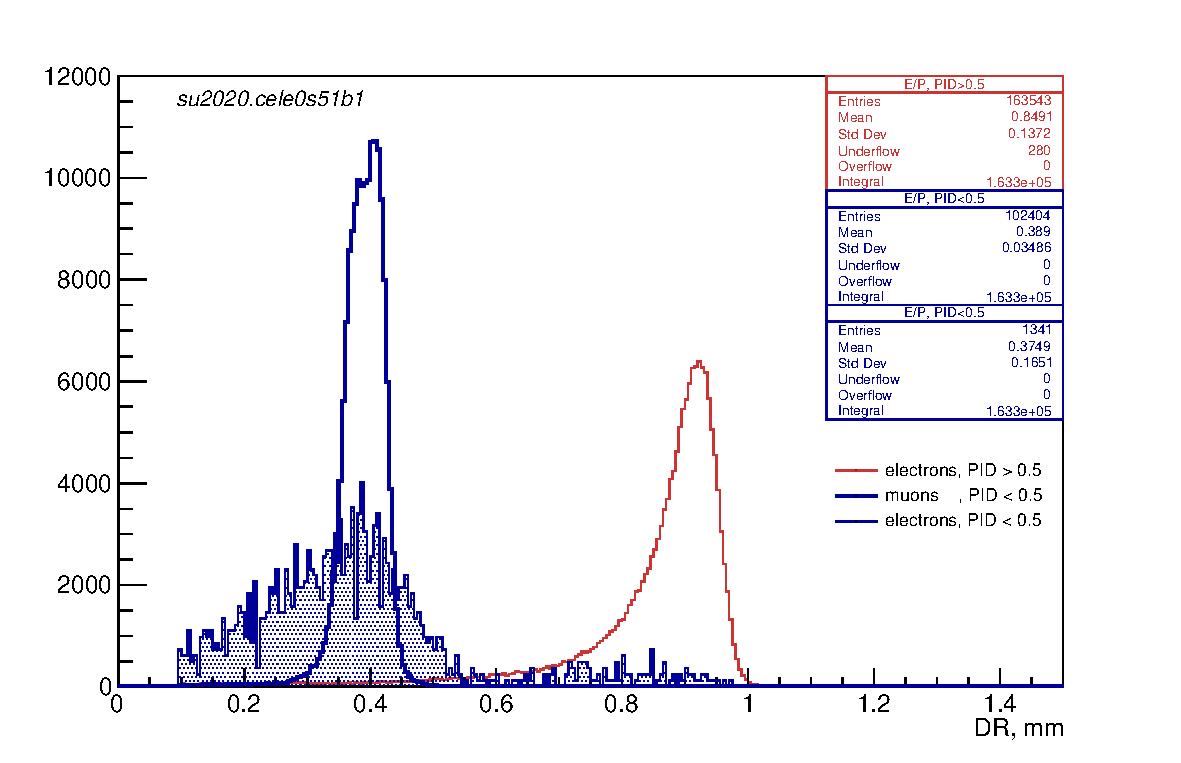
\includegraphics[width=0.80\textwidth]{figures/pdf/figure_00311_pid_emuana_trk_110_vs_111_ep}
      % }
    };
    \node[anchor=south west,inner sep=0] at (0,-7.0) {
      % \node[shift={(0 cm,0.cm)},inner sep=0,rotate={90}] at (0,0) {}
      % \makebox[\textwidth][c] {
      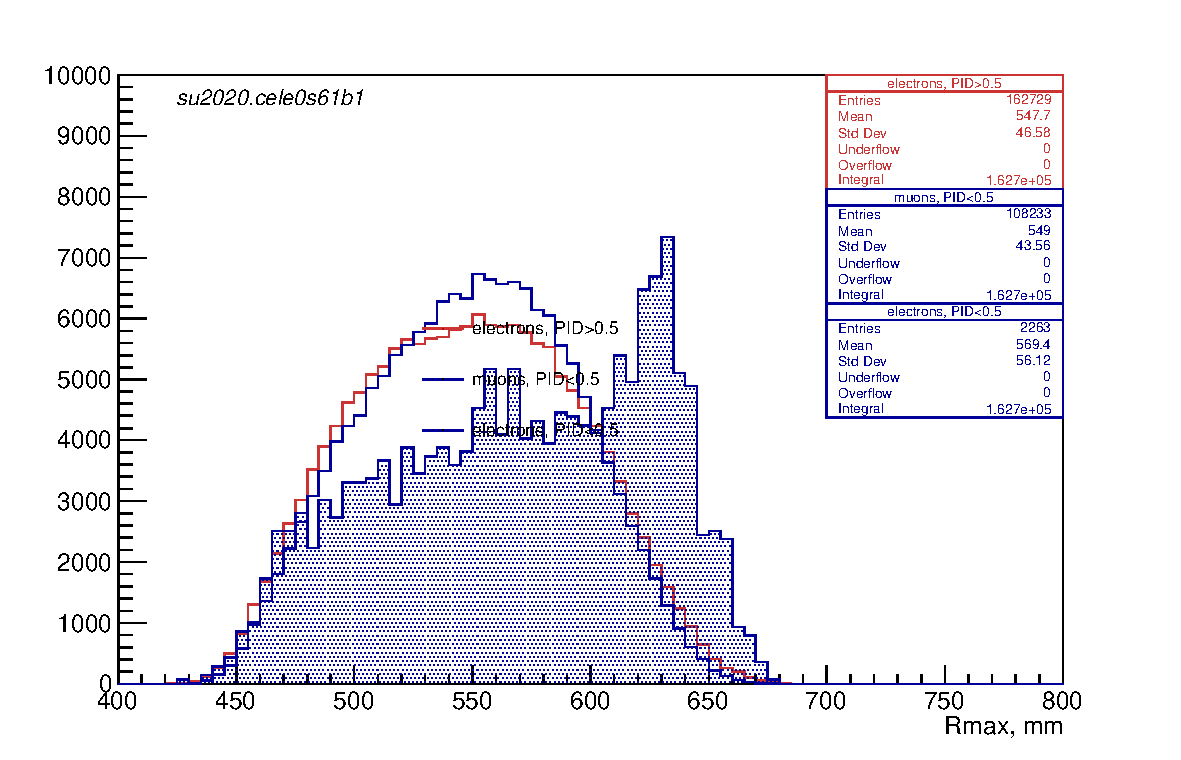
\includegraphics[width=0.80\textwidth]{figures/pdf/figure_00312_pid_emuana_trk_110_vs_111_rmax}
      % }
    };
    \node[anchor=south west,inner sep=0] at (10.3,-7.0) {
      % \node[shift={(0 cm,0.cm)},inner sep=0,rotate={90}] at (0,0) {}
      % \makebox[\textwidth][c] {
      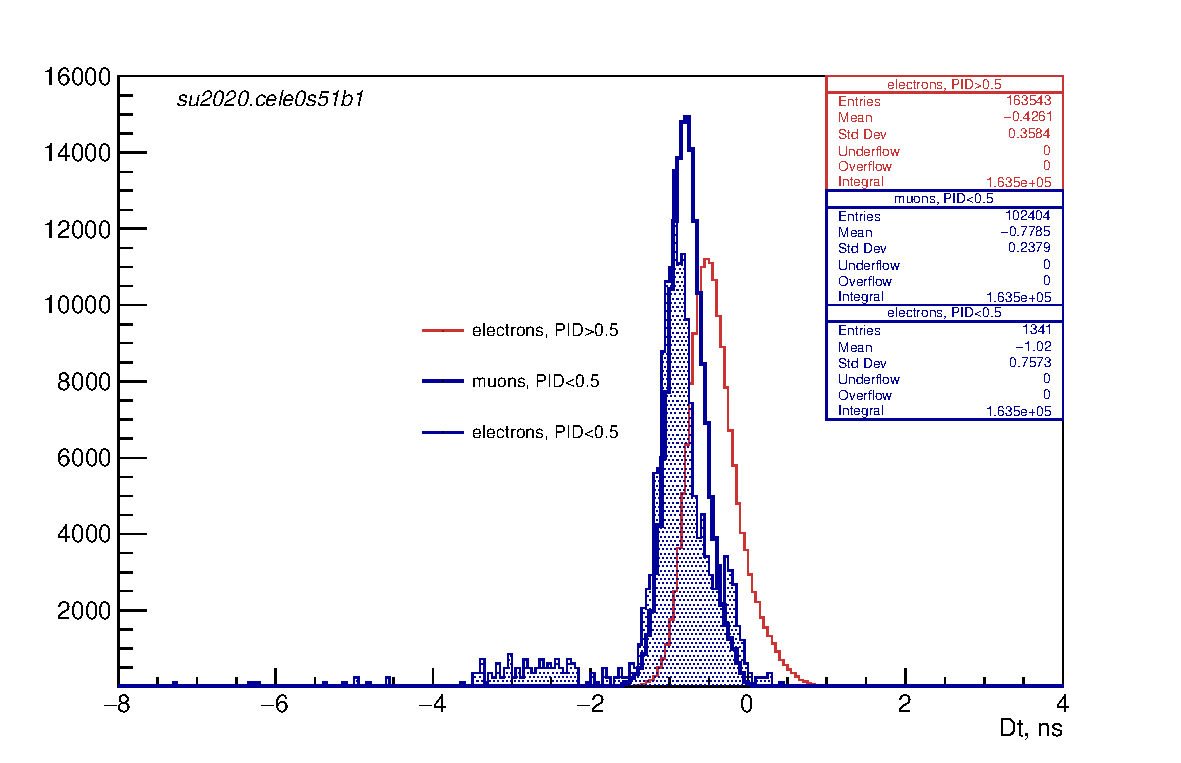
\includegraphics[width=0.80\textwidth]{figures/pdf/figure_00313_pid_emuana_trk_110_vs_111_tch_dt}
      % }
    };
    % \node [text width=6cm, scale=0.8] at (4.5,6.4) {mu2e-18894 by Kevin Lynch and Jim Popp};
  \end{tikzpicture}
  \captionof{figure} {
    \label{fig:electrons_failing_pid}
    % \caption{
    Distributions of the PID variables for electrons passing the PID, muons failing the PID, and electrons failing the PID.
    The PID selection used is $S_{PID} > 0.5$, where $S_{PID}$ is the value of the PID ANN score variable
  }
\end{figure}
